% \chapter{Introduction}\label{ch:introduction}
% Here is the introduction. The next chapter is chapter~\ref{ch:ch2label}.


% a new paragraph


\section{Examples}
You can also have examples in your document such as in example~\ref{ex:simple_example}.
\begin{example}{An Example of an Example}
  \label{ex:simple_example}
  Here is an example with some math
  \begin{equation}
    0 = \exp(i\pi)+1\ .
  \end{equation}
  You can adjust the colour and the line width in the {\tt macros.tex} file.
\end{example}

\section{Code example}
\begin{listing}[!ht]
\begin{minted}[
        frame=single,
        obeytabs=true,
        tabsize=1,
        linenos,
        numbersep=10pt,
        highlightlines={2},
        highlightcolor=newyellow]
        {c}
#include <stdio.h>
int main() {
   printf("Hello, World!"); /*printf() outputs the quoted string*/
   return 0;
}
\end{minted}
\caption{Hello World in C} \label{listing:2}
\end{listing}

asdasd asdasd  a asd 
\mint{html}|<h2>Code example here in text! <b>here</b></h2>|
asdasda 
asdasd



\chapter{Working at CERN}

This chapter will begin with a short introduction to CERN as an organisation, and afterwards describe my personal experience as a trainee.

\section{CERN as an organization}

CERN was established in 1954 by a multilateral intergovernmental treaty, better known as the CERN convention. 
It has four fundamental tasks:

\begin{itemize}
    \item \textbf{Research:} Seeking and finding answers about the universe
    \item \textbf{Technology:} Advancing the frontier of technology  
    \item \textbf{Collaboration:} Bringing nations together through science 
    \item \textbf{Education:} Training the scientists of tomorrow    
\end{itemize}
% \noindent CERN is divided into four sectors.

% \begin{itemize}
%     \item Accelerator and technology
%     \item Research and computing
%     \item International Relations
%     \item Finance and Human Resources
% \end{itemize}

% \noindent These sectors are further divided into eleven departments.

% \begin{itemize}
%     \item Site and Civil Engineering
%     \item Engineering
%     \item Theoretical Physics
%     \item Accelerator Systems
%     \item Information Technology
%     \item Technology
%     \item Beams
%     \item Experimental Physics
%     \item Industry, Procurement and Knowledge Transfer
%     \item Human Resources
%     \item Finance and Administrative Processes
% \end{itemize}

%%%%% Something about diversity  

\noindent Not only are CERN interested in technology and science, but also in collaboration and knowledge transferring between people. 
Diversity at CERN has been a core feature of the population since it was founded. CERN working towards an enviroment there includes peoples from all nationalities of its members. It is desired that many different nationalities comes together from around the world to learn, and to share their knowledge with each other. Here the diversity has a big value for CERN, and therefore it is important that CERN is appreciating differences and fostering equality to promote the collaboration and to create an inclusive work environment. The organization works towards an optimum-diverse workforce. From this, creativity and innovative from the collaboration between diverse ideas, perspectives and approaches unfolds.

Unfortunatly danish people are a minority at CERN. It's hard to get danish students to CERN because of the good conditions in Denmark. Derived from this problem CERN has established a Danish Student Program, to get more applicants from Denmark. 


To work abroad, and getting new knowledge and experience has high value for the individually and the nations. 

To transfer knowledge between nations has a great importance for the countries of the workers as well. The nations gets knowledge brought home by the workers, which can enhance development. 

\section{Work areas}

\subection{Involvement in internship}
In the internship my main purpose are developing of the EMP. The EMP is a processing platform targeting for applications in experiment for the HL-LHC. It serves as an interface between EMCI and the control room. The EMP is placed at non-radtion areas, where it serves as an optical link reciever. Further it supports connection with multiple VL+ to the front end.


\subection{The EMP}

The main task of this trainee has been to contribute to the development of the EMP. The EMP is based on a Trenz electronic carrier board - TE0808 \cite{TEBF080828:online}. 







Here I have contributed to configuration of the clock on the board. The clock need to be configured before it is able to communicate with the EMCI.



\subsection{Configuration of clock generator Si5345}
As the EMP boots there is a need to configure the clock before the EMP is able to communicate with the EMCI. The solution to this problem is to use Silabs ClockBuilder toolkit. The kit consists of an field programmer main board, which are connected to a PC via USB in one end, and the Trenz baseboard with a 10-pin female in the other end. This allow the user to easy configure the clock via a GUI software supported by Silabs - named Clockbuilder pro.

The problem with this solution is that the clock need to be reconfigured every time it boots. This makes the EMP dempendent of the Silabs Clockbuilder kit, and further not convenient for practical use. The setup is shown on figure \ref{fig:Silabstoolkit} below. 

\begin{figure}[H]
    \centering
    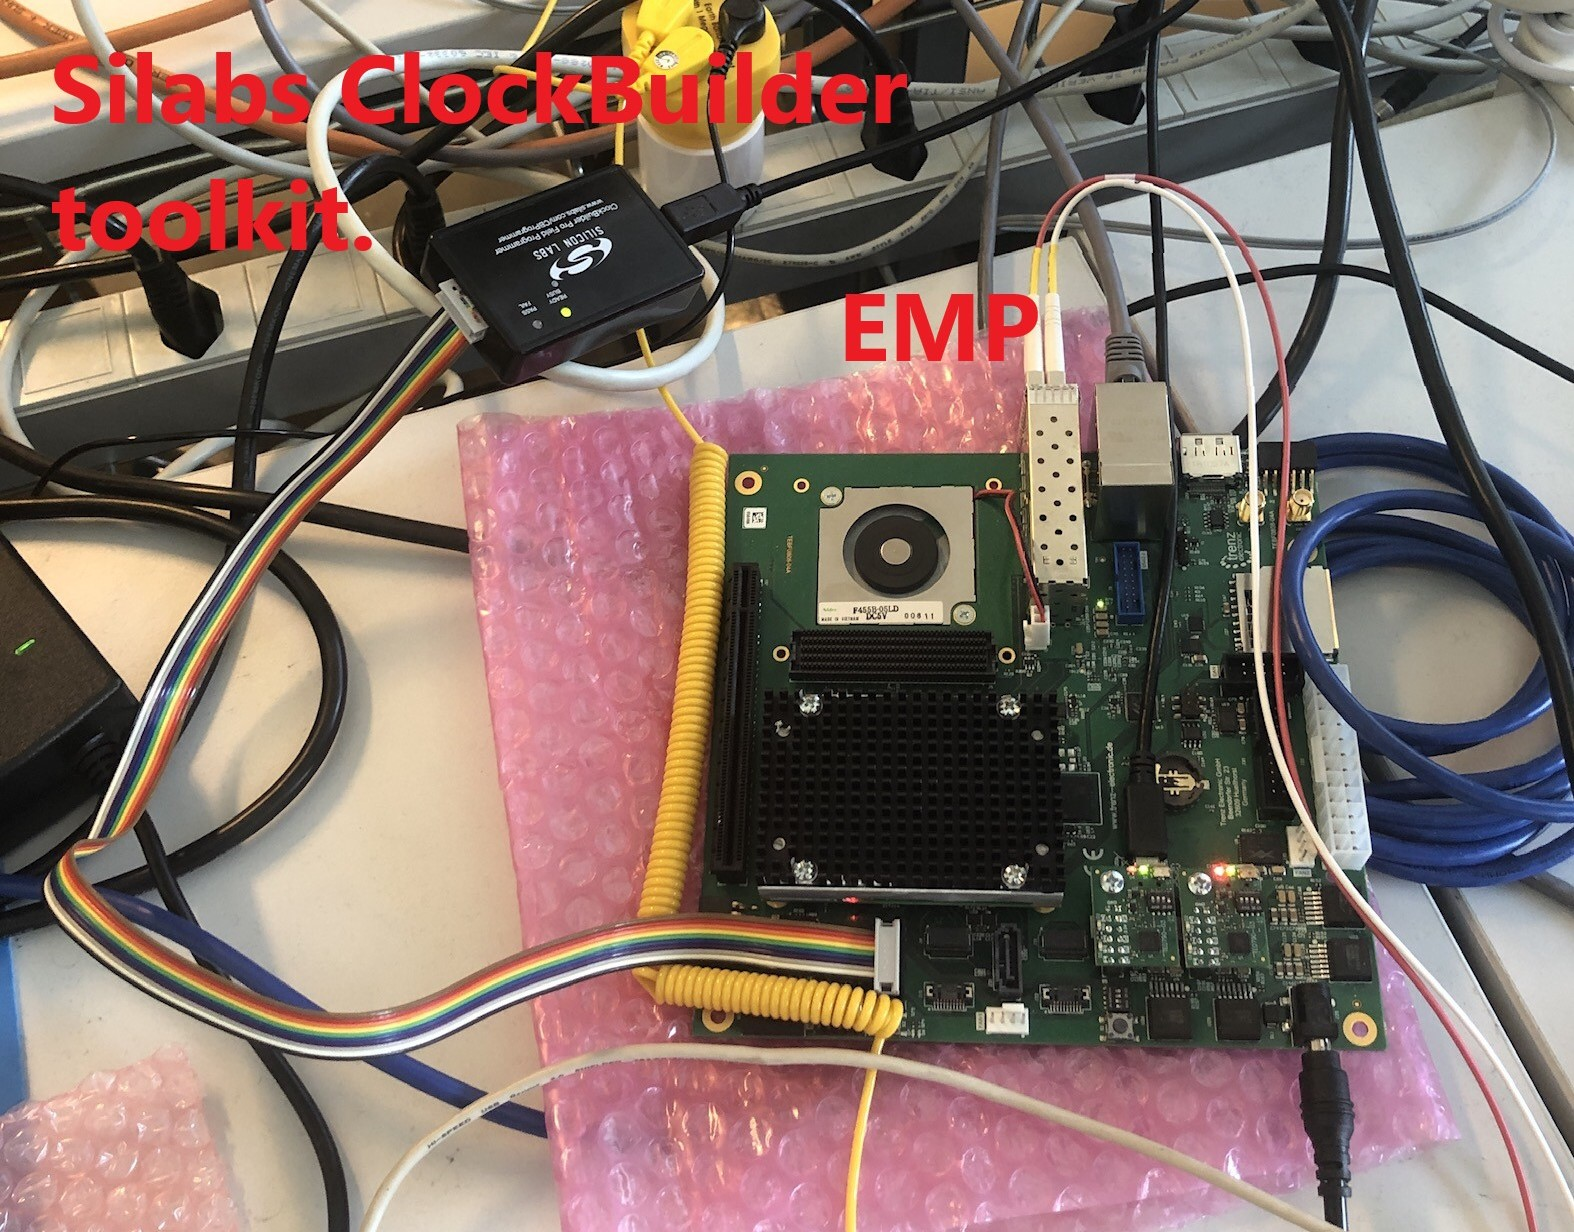
\includegraphics[width=.75\textwidth]{Graphics/IMG_0312.jpg}
    \caption{Setup of EMP connected to the Silabs toolkit.}
    \label{fig:Silabstoolkit}
\end{figure}


Another way to come around this problem is to make a program on the EMP which configure the clock itself. To do this the Xilinx Zynq Ultascale chip - which are placed on the Trenz baseboard - has to communicate with the On-module Quad programmable PLL clock generator Si5345 (TE0808). This is done with the use of I2C. In between the Xlinx chip and the clock generator is a 8-channel I2C switch (U27). From the manual it is found that the address to write to is 0x69 \cite{TEBF080828:online}. An overview from the manual is shown on figure \ref{fig:overview}.


\begin{figure}[H]
    \centering
    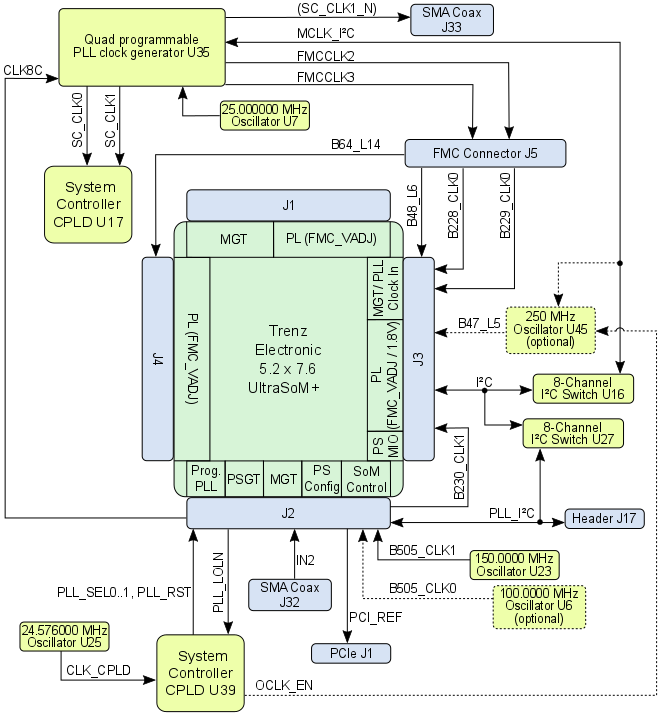
\includegraphics[width=.85\textwidth]{Graphics/BD-TEBF0808_Clocking.png}
    \caption{Overview of the clocking configuration on carrier board .}
    \label{fig:overview}
\end{figure}

Now that the slave address is known it is possible to write some code to communicate with the clock generator. The first thing to do in the code is to collect a list of registers and values to write to. Thankfully it is possible to export the configuration file from ClockBuilder to C, which makes it a lot easier. The file exported is shown i appendix \ref{app:B}. Now that we have the Data, we need to extract it in a way which suits the application. One problem here is that the register address is 16-bit, and that is a big problem because that the i2c only can handle 8-bit. This problem is solved by the register 0x0001. This register is a 'Page Register'. It allows us to select between 256 possible pages, and in that way to exceed 8-bit. To select a page - ex. page 1 - We have to write 0x01 to the register 0x01, and the page will be selected. The smart thing here is, that page 1 will start from the address where the previous page (0) endded. It means that page 0 start from address 0 and goes up to 255. Page 1 starts from address 256 and goes up to 511 and so on. So if we want to write to ex. register 0x0B24, we first have to select the page 0xB by writing 0xB to 0x01 (the Page Register), and then write to the address 0x24. In this way it is possible to write to 16-bit addresses, without exceed the data limit for the i2c of 8 bit.

\noindent For that reason the 16-bit register address given from the exported ClockBuilder file, has to be split into two 8-bit addresses. The upper 8-bit will be the value of the Page, and the lower 8-bit will be the value of the register address. This is not needed for the value extracted from the ClockBuilder file, since it is already 8-bit.


The function forging the data from the exported file is shown in listing \ref{listing:3}. The Function return an $n \times 3$ matrix, where the first column in the matrix is the value of the page. The second one is the value of the register, and the third one is the value to write, as shown here:\\  

\begin{figure}[H]
\centering
$\begin{vmatrix}
Page\:Address & Register\:Address & Value\\
\vdots & \vdots & \vdots\\
Page\:Address & Register\:address & Value
\end{vmatrix}$
\caption{$n \times 3$ Matrix returned by function \mintinline{html}{extractData()}.}
\end{figure}


\begin{listing}[H]
\begin{minted}[
        frame=single,
        obeytabs=true,
        tabsize=1,
        linenos,
        numbersep=10pt,
        highlightlines={},
        highlightcolor=newyellow]
        {c}
int **extractData() {

	uint8_t bytes[2];
	uint16_t addr;

	/* Numbers of elements in array */
	size_t array_size = sizeof(si5345_revb_registers)/8;

	/* allocating rows */
	int **arr=(int **)malloc(sizeof(int *)*array_size);

	/* initialize matrix: data_set[row][column] */
	int data_set[array_size][3];
	int column = 0 ;

	/* Writes data to matrix from Silabs design report */
	for (int row = 0 ; row < array_size ; ++row) {

			/* allocating columns */
			arr[row] = (int *)malloc(sizeof(int)*array_size);

			/* splits 16 bit into two 8-bits */
			addr = si5345_revb_registers[row].address;
			bytes[0] = addr >> 8; // high byte
			bytes[1] = addr & 0x00FF; // high byte

			/* writes address data first 8-bit to page column */
			arr[row][column] = bytes[0];
			
			/* writes address data last 8-bit to reg. addr. column */
			column=1;
			arr[row][column] = bytes[1];

			/* writes address data to thrid column for value 0xD8 */ 
			column=2;
			arr[row][column] = si5345_revb_registers[row].value;
			column=0;
	}
	return arr;
}
\end{minted}
\caption{The function extracting the data from the ClockBuilder file.} \label{listing:3}
\end{listing}


Now that the data is reachable, the I2C has to be setup. Here we use a code from Cosmin Tanisla\cite{linuxuse66:online}, to get started. The code has some great functions there will handle the I2C, and are easy to use. To setup the I2C create im creating a struct. The struct consist of a device filename and a device address. The filename is the path of the I2C bus file in the EMP, which is found on the EMP in the folder \mintinline{html}{/sys/class/i2c-dev/}. In this application we use the I2C-13. Further the device address was found in the Trenz baseboard manual as 0x69. The I2C device can now be started using the function from Cosmin Tanisla \mintinline{html}{i2c_start}, as shown at line 17 in the code snippet below \ref{listing:a}.

\begin{listing}[H]
\begin{minted}[
        frame=single,
        obeytabs=true,
        tabsize=1,
        linenos,
        numbersep=10pt,
        highlightlines={17},
        highlightcolor=newyellow]
        {c}
	int **data_from_emp_silabs;

	/* Fetching data from Silabs design report to an matrix */
	data_from_emp_silabs = extractData();

	/* Displays data in matrix */
	 show_data(data_from_emp_silabs);

	struct I2cDevice dev;

	/* Set the I2C bus filename and slave address,
	dev.filename = (char *)"/dev/i2c-13";

	/* clock generator Si5345 [U35] has slave address 0x69 */
	dev.addr = 0x69;

	i2c_start(&dev);
\end{minted}
\caption{The function extracting the data from the ClockBuilder file.} \label{listing:a}
\end{listing}


\noindent Now the I2C is setup, its possible to read/write data to the clock generator from the ClockBuilder file. The way this is implemented is with a \mintinline{html}{for loop}. The \mintinline{html}{for loop} starts from the first row of the matrix, fetching data from each column (i.e. page address, register address, value) and puts it into a corresponding 8-bit integer. This might not be necessary, but in my opinion it makes the code more readable. 
After the code is fetched into the corresponding variables, the value of the page is used in a switch case, its function is to manage which page to write to. After that, the register are written with value.
To validate that the writing is successful, the next sequence of code will read the data from the same register. If the value of the register matches, the value just written, it is confirmed that the register successfully has been written. But be aware of this is not always the case. Some registers are self clearing, and will therefore not have the value written - This must be taken into consideration when validating the data. When the register is written, the \mintinline{html}{for loop} do it all again, but for the next row - this continues until the matrix ends. This can be seen in the code snippet \ref{listing:ad}. The code snippet \ref{listing:ad} is not the actual code used, though, but is a shortened version, to give the reader the basic idea of the essential concept. The actually code used is shown in appendix \ref{app:C}.

\begin{listing}[H]
\begin{minted}[
        frame=single,
        obeytabs=true,
        tabsize=5,
        linenos,
        numbersep=10pt,
        highlightlines={},
        highlightcolor=newyellow]
        {c}
/* Calculate size of array from EMP_Silabs */
size_t array_size = size_of_array() - 1;
for (int i = 0; i < array_size; ++i)
{
	/* Fetch data from matrix */
	uint8_t page = data_from_emp_silabs[i][0];
	uint8_t reg = data_from_emp_silabs[i][1];
	uint8_t value = data_from_emp_silabs[i][2];
	switch (page)
	{
	case 0:
		i2c_write_reg(&dev, 0x01, 0x00);
		break;
    /* from 0 up to 11 */
	case 11:
		i2c_write_reg(&dev, 0x01, 0x0B);
		break;
	default:
		return -1;
	}
	i2c_write_reg(&dev, reg, value);
}
i2c_stop(&dev);
return 0;

\end{minted}
\caption{Trimmed version of the code in appendix \ref{app:C}. Describes the essential functionality of the code used for fetching data and writing it into registers.} \label{listing:ad}
\end{listing}

When the code is executed it displays every register written. with the related information of page, register address, current value and written value, and most importantly, if the process succeeded. Further the output gives insight in the phases of the writing. As mention earlier, the configuration has to follow a certain sequence. This sequence are split into three phases: The preamble, the registers to be written, and the postable. A code snippet is shown in listing \ref{listing:4}.

\begin{listing}[H]
\begin{minted}[
        frame=single,
        obeytabs=true,
        tabsize=1,
        numbersep=12pt,
        highlightlines={},
        highlightcolor=newyellow]
        {bash}
Start configuration preamble
*********************************************************************
  Action:       Page:   Register:   Value:    Writing:     Status:
*********************************************************************
  [Wrote]        B       0x24        0xDB      0xD8       [Success]
  [Wrote]        B       0x25        0x2       0x0        [Success]
  [Wrote]        5       0x40        0x0       0x1        [Success]
*********************************************************************

 Start configuration registers
*********************************************************************
  Action:       Page:     Register:   Value:    Writing:     Status:
*********************************************************************
[Overwrote]      0       0xB         0x68      0x68       [Success]
[Overwrote]      0       0x16        0x2       0x2        [Success]
[Overwrote]      0       0x17        0x1C      0x1C       [Success]
[Overwrote]      0       0x18        0xEE      0xEE       [Success]
   ...          ...      ...         ...        ...          ...
\end{minted}
\caption{Code snippet of the output when the program is executed} \label{listing:4}
\end{listing}

One thing that hasn't been explained yet, is the data from the ClockBuilder file. When writing to the clock generator it is important to know the properties of the registers (ex. the Page Register) writing to. For this I used the datasheet for Si5345 rev. D family \cite{Si5345Si17:online}. This is important to follow, because reprogramming can make the clock programmer unresponsive. Of the same reason, every time any change causes the VCO (Voltage Controlled Oscillator) frequency to change by a threshold of 250 PPM deffernce from the power-up. It require a special sequences of writes to registers. These are instructions are listed in the datasheet, but be aware of the clock generator used in this project is Rev B, and not the Rev D. This means there are small changes, and one of them is in this particular sequence.



\subsection{dsdf}



The code is built upon a code from Cosmin Tanisla\cite{linuxuse66:online}.


is connected to a pin header (J17)






synchronisation of clock between the EMP and EMCI. 









with the tasks of trying to make a program there could easily configure the clock. The task are in my opinion perfect, I get involved in a lot of the aspects of the project, hereby 

thereby also gaining opportunity of learning much more.




The GUI which will be the users interaction with the program, are being developed i Python, and language which was new to me. The GUI has to run at a remote PC, since the EMP not are capable of running programs which demanding high resources. The EMP however, has to execute the code. So the solution i came up with was a server/client relationship between the remote PC and the EMP, where the GUI is implemented a the remote PC (as server), and a C++ code is implemented in the EMP (as client) to execute the actually code. The C++ code is 








\chapter{Relevant work areas at internship}

All programming done at Aalborg University are related in many ways to the work i has done at CERN.

Knowledges about programming languages beforehand has great influence in the learning of new programming languages
such as Python. Further concepts like multi-threading, semaphores and mutex has also been relevant throughout this internship.

\section*{Hardware used:}
\begin{description}
    \item[EMP]  Embedded Monitoring Processor
    \item[EMCI] aadsda asd ass
\end{description}

\section*{Software used:}
\begin{description}
    \item[Vivado] Embedded asd asda d
    \item[Vitis] aadsda asd ass
\end{description}

\section{Definitions:}

\begin{description}
    \item[Embedded Software Development] The developement of creating a software platform from the hardware platform and develop the application code using the embedded CPU.
    \item[Board Support Package (BSP)] 
    \item[Image]

    \item[AXI]
    \item[Virtual memory]
    \item[]
    
\end{description}

\section{EMCI}

The EMCI is designed to be radition tolerant, as it usually is placed in a radioctive enviroment. 

EMCI is designed to be radiation tolerant, 

\section{EMP}

The EMP is the counter part of the EMCI and is not radiation tolerant. It's act as a processor for the EMCI, which communicates with several FE's in the detector.


It can manage up to 12 EMCI's in a star topology. 

The EMP is via ethernet controlled from the back-end 

\subsection{Based on}
It is based on a Xilinx Zynq Ultrascale+ MPSoC with a ARM multi-core processor. 

\subsection{The PS }


\section{PetaLinux}

PetaLinux is used for customization, building and deploying Embedded Linux solutions on Xilinx processing systems. It is an embedded Linux Software Development Kit to handle the FPGA-based system design on an SoC. In this case, it will be targeting the UltraScale+ Xilinx MPSoC with the firmware. 

PetaLinux 



\section{Problem analysis}
\section{Theory}
\section{Methods}
\section{Models}
\section{Solution suggestions?}
\section{Implementation}
\section{Tests}
\section{Conclusion}
\section{m.m.}

\chapter{Analysis of internship}
\section{Professionally}
\section{Work related}
\section{Social}